
\section*{Health}
\DefineNamedColor{named}{eclipsered}{rgb}{0.186,0.566,0.182}
\definecolor{tablecolor}{named}{eclipsered}

\subsection*{Physical Health}

\begin{eptable}{ X }
   \epheader{1}{Wounds}
   Each wound causes cumulative \modifier{-10} on all tests, \modifier{-1} to initiative.\\
   When receiving wound, \skill{SOM} or knockdown.\\
   When receiving 2x wound at once, automatic knockdown. \skill{SOM} or unconscious.\\
\end{eptable}

\begin{itemize}
    \itembox If character suffered wound and damage exceed DUR they are in
            danger of bleeding out. Make \skill{SOM}. On failure receive
            \dv{1} per wound per turn until dead or stabilized with \skill{Medicine: Paramedic}.
\end{itemize}

\bigskip

\begin{figure}[htbp!]%
   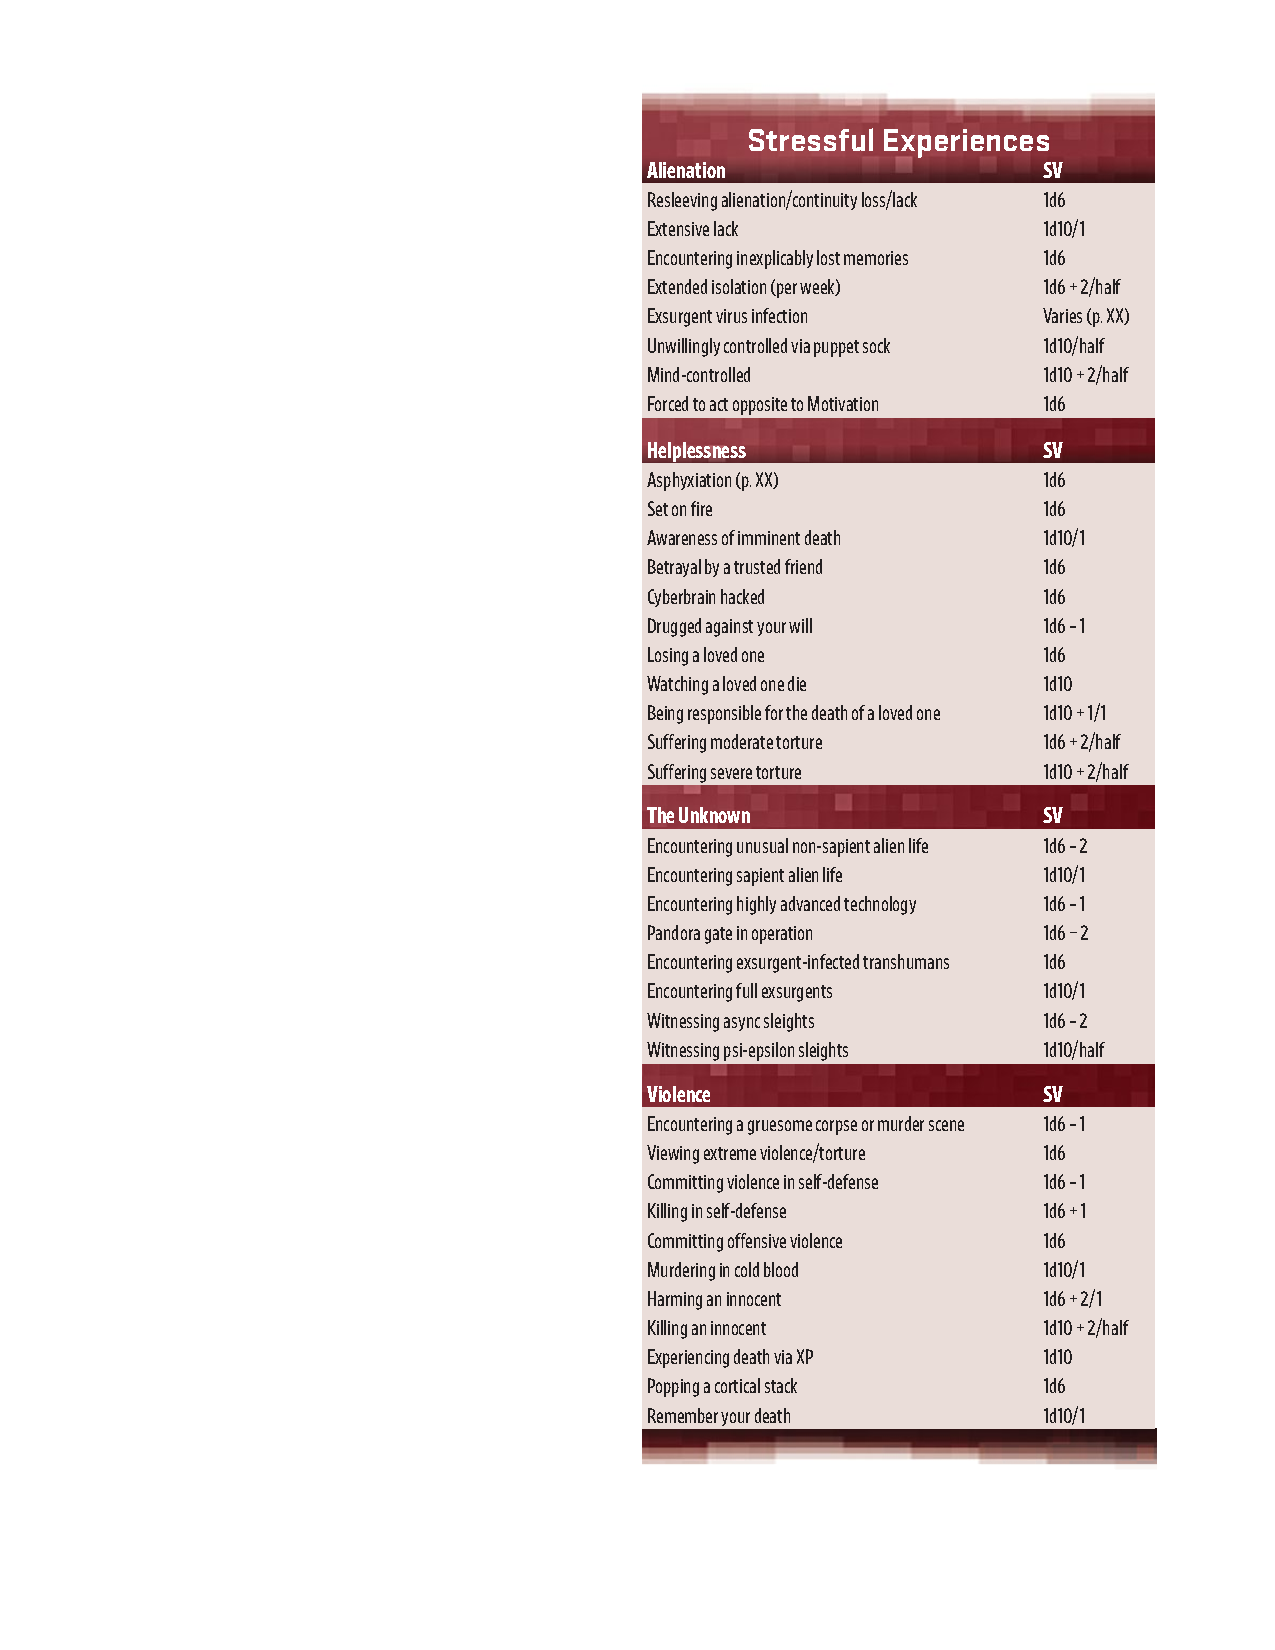
\includegraphics[scale=0.82]{gfx/health-stress}%
\end{figure}%

\begin{eptable}{ l | X | X }
   \epheader{3}{First Aid}
   Medicine: Paramedic & 1 wnd. and \dv{1d10} & \SI{10}{min} + 10 per wnd.\\
\end{eptable}

\bigskip

\begin{eptable}{ l | X | X }
   \epheader{3}{Healing}
   No Biomods & \dv{1d10} per day & 1 wound per week.\\
   Biomods & \dv{1d10} per \SI{12}{h} & 1 wound per 3 days.\\
   Medichines & \dv{1d10} per \SI{1}{h} & 1 wound per 1 days.\\
   Nanobandages (max 3) & \dv{1d10} per \SI{1}{h} & 1 wound per 1 days.\\
   Healing Vat & \dv{2d10} per \SI{1}{h} & 1 wound per 2 hours.\\
   Poor Conditions & x2 & x2\\
   Harsh Conditions & x3 & x3\\
\end{eptable}

\begin{itemize}
    \itembox All damage must be healed first before wounds can be healed!
    \itembox Medicine: Paramedic is exception as it heals both
            at same time. Can only be used once per set of
            injuries. Only within first 24 hours.
\end{itemize}


\bigskip

\subsection*{Mental Health}


\begin{eptable}{ l | X }
   \epheader{2}{Stress Sources}
   Alienation & Disconnection to the self, loss of self.\\
   Helplessness & Inability to control events, betrayal.\\
   The Unknown & Anything alien.\\
   Violence & Threats and harm to self and others.\\
\end{eptable}

\bigskip


\begin{eptable}{ X }
   \epheader{1}{Stressful Experience}
   When encountering something horrific \skill{WIL} check.\\
   On failure receive stress as indiciated on table.\\
   On each trauma, take note of event on character sheet.\\
   Receiving \num{5} traumas w.o. receiving disorder, character hardens.\\
   Hardening permanently gives \modifier{-10} to WIL Checks and Persuade.\\
\end{eptable}

\begin{itemize}
    \itembox Disorders are received by stress exceeding lucidity.
    \itembox Disorders are triggered by traumas or circumstances.
\end{itemize}

\bigskip

\begin{eptable}{ X }
   \epheader{1}{Traumas}
   Each trauma causes cumulative \modifier{-10} on all tests, \modifier{-1} to initiative.\\
   Receiving trauma, \skill{WIL} or stunned, shake w. cmplx. action. Triggers disorder.\\
   Receiving 2x trauma at once, automatic stunned. \skill{SOM} or ASR.\\
   ASR: Attack OR Flee OR Detach. Friends can try \skill[-30]{Provoke} to snap out.\\
\end{eptable}

\begin{itemize}
    \itembox Traumas trigger disorder of the same type they are from. Players encouraged to role play reactions.
    \itembox To recall later what happened \skill[-30]{COG} check.
    \itembox Accute Stress Responses (ASR) determined randomly. Player remains in mode until incapacitated, threat avoided, destroyed or snapped out.
\end{itemize}


\bigskip


\begin{eptable}{ l | X }
   \epheader{2}{Disorders}
   % Addiction & Needs fix or receive negative modifier.\\
   Alien Behavior Disorder & Prone to exhibiting alien behavior.\\
   Anxiety & Needs to be convinced to do almost anything.\\
   Atavism & Show primitive or animalistic behavior.\\
   ADHD & Negative perception modifier and task effects.\\
   Autophagy & Consume yourself.\\
   Bipolar & Prone to risky behavior.\\
   Body Dysmorphia & Prone to alienation.\\
   Cosmic Anxiety Disorder & Flee from aliens / TITANs. \\
   Conversion Disorder & Blindness, deafness, loss of balance, ...\\
   Depression & Requires test to take any action. \\
   DPD & Separate personality. \\
   Fugue & Totally non-responsive. \\
   Impulse Control & Engage in activity that controls thoughts. \\
   Insomnia & Long rests become short, no short. Bad perception.\\
   Narcissistic PD & Demand attention.\\
   Paramnesia & Recall memories not own, confused about self. \\
   Paranoia & Expect betrayal everywhere. \\
   Phobia & Try to avoid phobia's focus. \\
   PTSD & Respond to triggers with violence. \\
   Schizophrenia & Experience delusions and hallucinations. \\
\end{eptable}

\begin{itemize}
    \itembox Effects are often resisted by \skill{WIL} tests for one or a few rounds.
\end{itemize}


\bigskip

\begin{eptable}{ X }
   \epheader{1}{Psychic Care}
   Psychic care is delivered by Medicine: Psychosurgery or Know: Psychology.\\
   Healing \sv{1d6} stress is task action (\num{1} day*).\\
   Healing 1 trauma is task action (\num{8} days*).\\
   Healing 1 disorder is task action (\num{40} days*).\\
   Each trauma and disorder applies \modifier{-10} to test.\\
   *Only \num{1} effective hour of treatment needed a day, \eg, trauma: 8 days, 1h each.\\
\end{eptable}

\begin{itemize}
    \itembox If patient receives new stress during treatment, it must be restarted.
    \itembox If VR is used, each hour of healing still requires full simulated day for person.
    \itembox Healing naturally, players can make \skill{INT} each month they didn't get new
            stress, healing \sv{1d6} or \num{1} trauma. Disorders require \num{3} months.
\end{itemize}


\begin{figure}[htbp!]%
   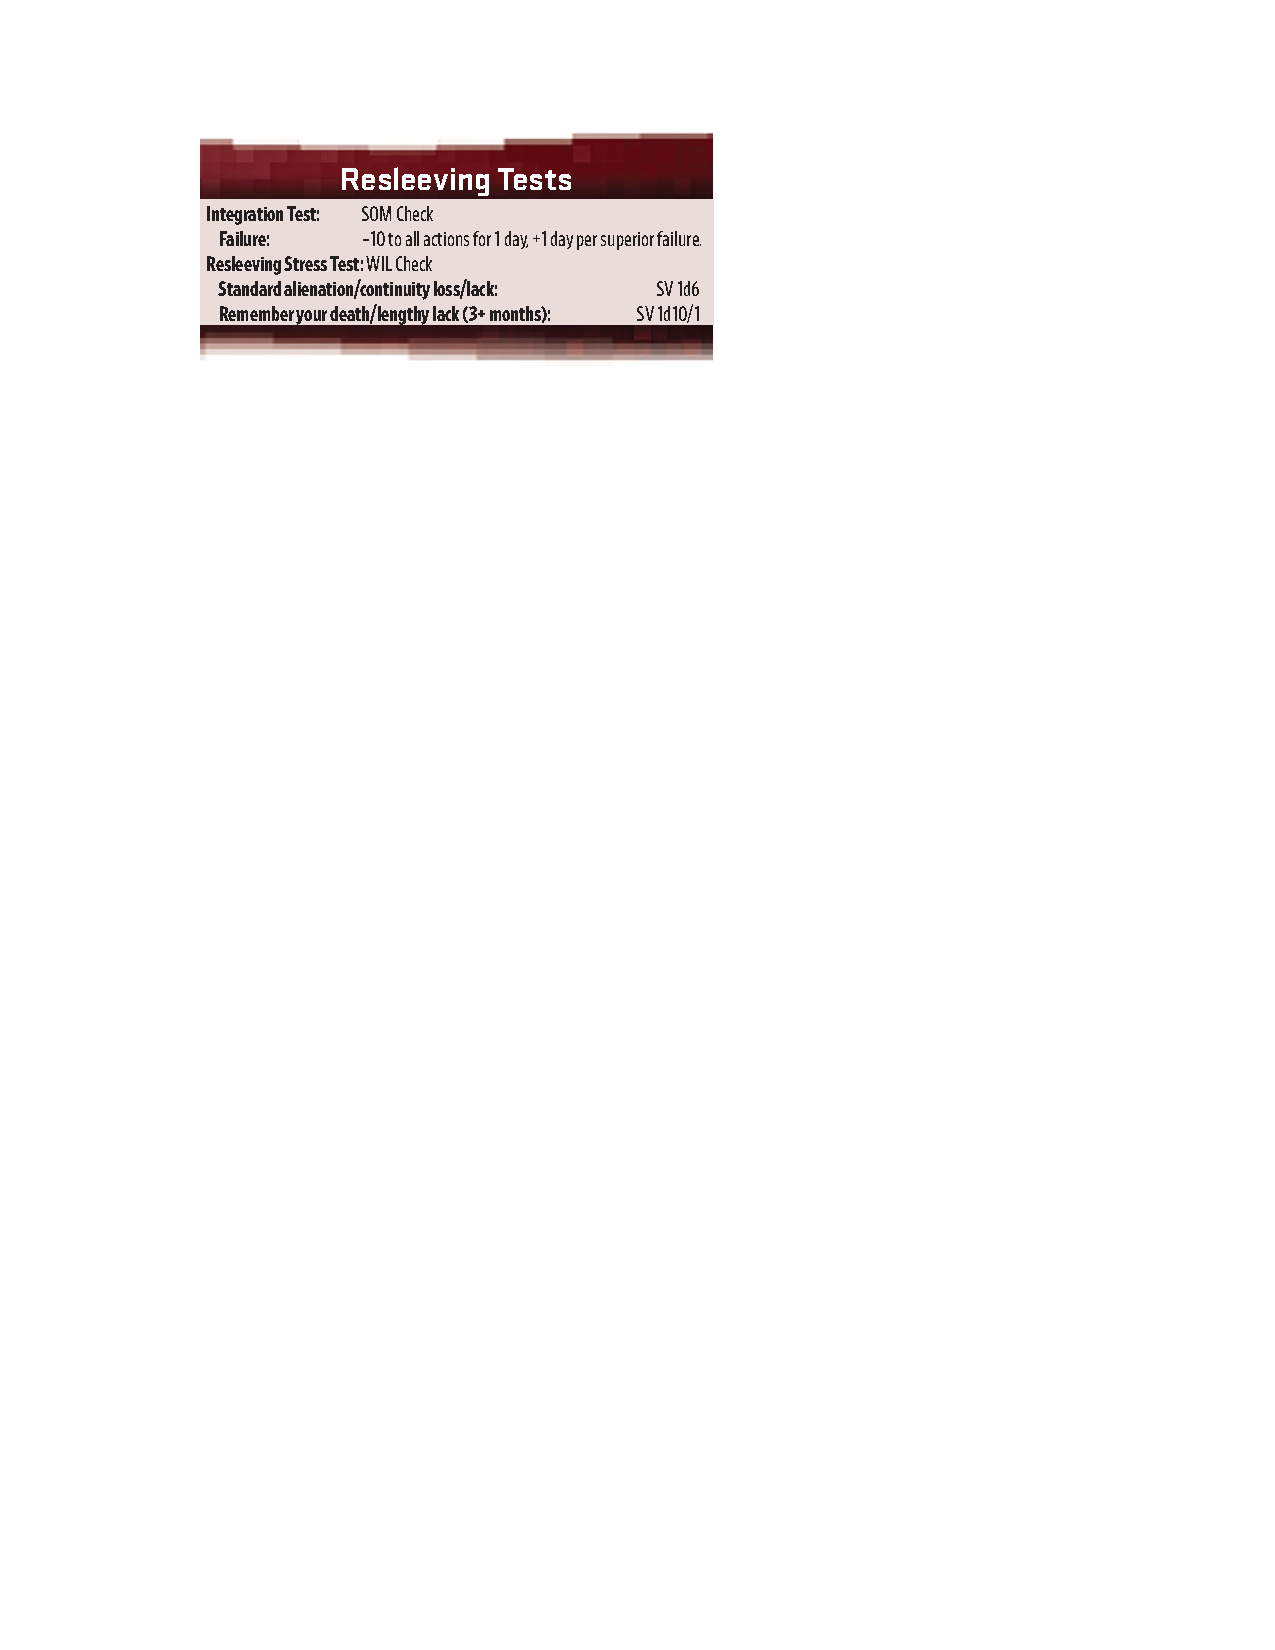
\includegraphics[scale=0.84]{gfx/health-resleeving}%
\end{figure}%
